\chapter{Methods}

\section{Experimental measurements of intercalation}

(~for example through displacement assays (move to experimental section, experimental difficulties, why is it hard to measure DNA intercalator biding affinity)~). ~Here we looked at a congeneric series intercalators based on a common quinoxaline scaffold with experimental measurements \cite{}.(Move to methods)~

\begin{figure}[h]
	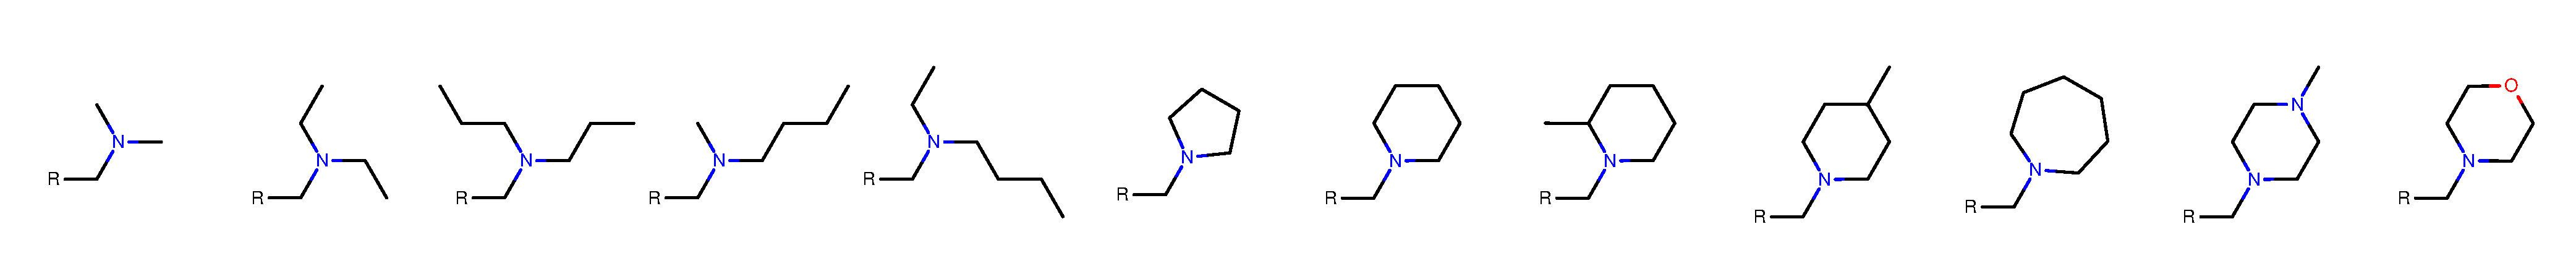
\includegraphics[width=\textwidth]{intercalators.pdf}
	\caption{A congeneric series of DNA intercalators. All molecules share a common quinoxaline scaffold. ~The experimental study was conducted by \cite{} producing binding affinity values that we could compare our calculations to. (Mention it in the experimental section)~ }
	\label{fig:intercalators}
\end{figure}


\section{Docking and scoring}

For certain application, like that of high throughput screening in the pharmaceutical industry, it is important to assess the binding strenght of a large number of drugs or molecules bound to large biological macromolecules like proteins or DNA in a very fast manner. This is done via easily evalutable scoring function, some notable examples including: AutoDock, X-Score, DrugScore, ChemScore, GOLD, FlexX, LigScore and LUDI. Generally speaking, they take into account a single structure and little or no protein movement is taking into account during evaluation. One of the simplest scoring function  consists of the empirical surface-area based method that shows that ligand binding reduces the surface are in the receptor that is accessible to the surrounding solvent. The function makes the assumption that the polar and non-polar area on the surface of the molecule has a linear relation to the free energy. Due to the crude simplifications in these models, they have weak predictive power and are rarely used for accurate free energy estimation. Here, a scoring methods is used for two reasons: (i) to find an initial structure for the intercalator-DNA complex, and (ii) to compare the scores and hence the ranking of this methods with other, more accurate models. Docking and scoring has its place in the drug discovery pipeline. In high throughput scenarios, where speed is an important factor due to the large number of molecules that need to be tested, scoring functions are often used to filter out candidates that have low probability of being good binders.

\subsection{Starting structures for docking}



\subsection{MMPBSA}

Molecular Mechanics Poisson-Boltzmann Surface Area (MMPBSA) is one of the theoretically approximate methods to calculate the free energy of system \cite{gilson2007calculation, steinbrecher2010towards}. It is the most accurate of the approximate methods, and it has previously been applied successfully to the free energy calculation of various biological systems including protein-ligand and DNA intercalator complexes.

This method is a good choice for comparing and ranking a set of molecule by their binding affinities for two main reasons: MMPBSA is able to handle a wide variety of systems and can the results can be theoretically calculated from a a single trajectory, unlike theoretically exact alchemical methods like FEP or TI. 

MMPBSA has become the a popular method to calculate binding affinities because of a balance between the details included in the physical model and the speed of the calculations themselves \cite{kollman2000calculating, sitkoff1994accurate}. As one of the main methods used in this thesis to calculate DNA-intercalator interactions, it will be discussed in more detail.

Applying the MMPBSA method to a system involves calculating the absolute free energy of binding by calculating three separate components: the free energies of the DNA-intercalator complex, the DNA and the intercalator molecules alone. The change is free energy upon intercalation then is

\begin{equation}
  \Delta G = \langle G_{complex} \rangle - \langle G_{DNA} \rangle - \langle G_{intercalator} \rangle
\end{equation}
\label{eq:mmpbsa}

where $\langle \dots \rangle$ represent the average value of a post-processing calculation performed on every frame of the simulation trajectory. Simulations are performed in explicit solvent and with counter-ions to balance the charge in the periodic simulation box.
To aid faster convergence of the free energy values the MMPBSA methods employs two strategies: first, all solvent molecules and counter-ions are replaced from the trajectory post simulation but pre-analysis by a continuum solvent approximation, and a thermodynamic cycle is used.

\subsubsection{The thermodynamic cycle}

\begin{figure}
  \centering
  \begin{tikzpicture}
  [ 
  waterbox/.style={rectangle,draw=blue!50,fill=blue!10,thick, inner sep=0pt,minimum size=5*\r},
  dna/.style={ultra thick, line cap=round},
  intercalator/.style={dna, dna, line width=3pt, blue},
  pre/.style={<-,shorten <=1pt,shorten >=1pt,semithick}, 
  post/.style={->,shorten <=1pt,shorten >=1pt,semithick}
  ]
  
  \node[waterbox] (a)               {};
  \node[waterbox] (b)  [right=of a] {}
    edge [pre] node[auto, swap] {$\Delta G_\text{b}^{aq}$} (a);
  \node[waterbox, fill=white] (a') [below=of a] {}
    edge [post] node[auto] {$\Delta G_\text{intercalator}^{sol}$} (a);
  \node[waterbox, fill=white] (b') [below=of b] {}
    edge [pre] node[auto] {$\Delta G_\text{b}^{vac}$} (a')
    edge [post] node[auto] {$\Delta G_\text{complex}^{sol}$} (b);
  \node[waterbox] (c)  [left=of a] {};
  \node[waterbox, fill=white] (c') [left=of a'] {}
    edge [post] node[auto] {$\Delta G_\text{dna}^{sol}$} (c);
    
  \node at ($(c.center)!0.5!(a.center)$) {+};
  \node at ($(c'.center)!0.5!(a'.center)$) {+};
  
  % \node[text width=10cm, align=center] [above=of a] {Thermodynamic cycle used to indirectly calculate the absolute free energy of intercalation};
  
  
  \foreach \x in {b.center, b'.center, c.center, c'.center} {
    \draw[dna]
      (\x) [rounded corners=\r] -- ++(-\s, 0) -- ++(0, 2*\s) 
      (\x) [rounded corners=\r] -- ++( \s, 0) -- ++(0, 2*\s)
      (\x) [rounded corners=\r] -- ++(-\s, 0) -- ++(0,-2*\s)
      (\x) [rounded corners=\r] -- ++( \s, 0) -- ++(0,-2*\s)
      
      (\x) ++(-0.866*\s,  0.5*\s) -- ++(1.73205*\s, 0)
      (\x) ++(   -\s,      \s) -- ++(   2*\s, 0)
      (\x) ++(   -\s,  1.5*\s) -- ++(   2*\s, 0)
      
      (\x) ++(-0.866*\s,  -0.5*\s) -- ++(1.73205*\s, 0)
      (\x) ++(      -\s,      -\s) -- ++(      2*\s, 0)
      (\x) ++(      -\s,  -1.5*\s) -- ++(      2*\s, 0);
  }
  
  \draw[intercalator] (a.center)  ++(-0.8*\s, 1.25*\s) -- ++(1.6*\s, 0);
  \draw[intercalator] (b.center)  ++(-0.8*\s, 1.25*\s) -- ++(1.6*\s, 0);
  \draw[intercalator] (a'.center) ++(-0.8*\s, 1.25*\s) -- ++(1.6*\s, 0);
  \draw[intercalator] (b'.center) ++(-0.8*\s, 1.25*\s) -- ++(1.6*\s, 0);

\end{tikzpicture}
  \caption{A solvation thermodynamic cycle is used to indirectly calculate the absolute binding free energy, $\Delta G_{b}^{aq}$, of an intercalator to the DNA in solvent. The rest of the free energy changes are calculated or estimated to then compute free energy of intercalation.}
  \label{fig:mmpbsacycle}
\end{figure}


\subsubsection{Single and Component trajectories}

The different contributions in equation \ref{eq:mmpbsa} can be extracted from a single trajectory of the complex, or from separate trajectories of the DNA, intercalator and complex. If a single trajectory is used, then the during the calculation of the different component, the rest of the system is removed and the analysis is done on part of the trajectory. This approach is effective in most scenarios and saves the additional cost of running multiple simulations for the separate components\cite{foloppe2006towards, wang2001use}. The other advantage of the single trajectory approach is that part of the complex that do not affect the intercalation cancel out exactly, as the coordinates are taken from the same trajectory, hence they are exactly the same. If separate trajectories are run for each component, than this error cancellation does not occur, as the component are free to explore different conformations. On the other hand, a single trajectory will not be able to capture dynamical changes to either the intercalator or, more importantly to the DNA, upon intercalation, and will consequently ignore certain contributions to the binding free energy. In the rest of the thesis, the three possible trajectory approaches are termed 1, 2 and 3 trajectory, corresponding to MMPBSA calculations where all three components are from the same simulation (1 trajectory), the intercalator is from a separate simulation (2 trajectory), or all three components, including the DNA are from three separate simulations (3 trajectory). 


\section{TIES}

The complexes of target DNA and hybrid intercalators were solvated in an orthorhombic water box with buffer width of 11 angstrom. The system was neutralized electrostatically with counterions. The BSC1\cite{ivani2016parmbsc1} force field was employed in all our simulations for DNA parameters. Intercalator parameters were produced using the general AMBER force field 2 (GAFF2) \cite{wang2004development}. The AM1BCC \cite{jakalian2002fast} %
semi-empirical methods was used to produce the partial charges on the intercalator atoms (AmberTools 18 \cite{ambertools18}) after geometry optimization with the OpenEye OEGauss toolkit. The simulation engine NAMD 2.12 was used for producing all the trajectories of the complex systems with periodic boundary conditions. The system was brought to and maintained at a temperature of 300 K and 1 atmosphere using the NAMD implementation of the Langevin thermostat (with a damping coefficient of $5 ps^{-1}$) and a Berendsen barostat (compressibility of $4.57 \times 10^{-5} bar^{-1}$ and a relaxation time of $100 fs$). The time step was set to $2 fs$. The van der walls terms perturbed linearly with respect to $\lambda$. To avoid end point catastrophes were atoms near the end point appear suddenly too close to each other a soft core potential was used for the van der Walls interactions. The electrostatic interactions of the disappearing atoms are linearly decoupled until $\lambda = 0.55$ then completely turned off afterwards, and those atoms that are appearing are electrostatically turned on from $\lambda = 0.45$ linearly increasing until the end.

All calculations were done with 13 $\lambda$ windows. At each value of $\lambda$ 5 replica simulations were run to assess the error. For each replica, the standard protocol for minimisation and equilibration was performed, that is 4 ns of simulation time. Production runs for each replica were 16 ns long. While the coordinates were recorded every 10 ps, $\partial V / \partial \lambda$ values were recorded every 2 ps. The choice of 16 ns for the simulation length and 5 for the ensemble size is based on the uncertainty quantification and error analysis discussed in the previous work. The protocol described here can be adjusted to the specific system at hand, but this was enough to converge results for all of the systems in this study. The size of the ensemble can be adjusted even at specific windows to account for additionally uncertainty that may arise. The TIES workflow can be executed in an embarrassingly parallel fashion, and given sufficient resources the simulations can finish in 15 hours. In general the turnaround time depends on the system size, number of cores used per simulation instance with GPUs offering additional speedup.

